\setcounter{section}{36}
\section{Нахождение точек сочленения в неориентированном графе.}
Пусть v - вершина графа, \textbf{не являющаяся корнем}, (v, to) - какое-то древесное ребро из вершинки v.\\  v - точка сочленения $\Longleftrightarrow$  ret[to] $\geq$ tin[v]
\begin{center}
    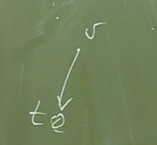
\includegraphics[width=3cm]{images/37_alg22.PNG}
\end{center}
$\blacktriangle$
$\leftarrow \ $Это условие понятно интуитивно. Если при спуске ниже v лучшее, чего мы можем добиться - вернуться в v, то если мы исключим вершину v, не сможем вернуться из поддерева в предков v, а значит, связность нарушится
\\
\\
$\rightarrow \ $ предположим, ни для какого сына неравенство не выполянется. Тогда  ret[to] < tin[v], а значит из каждого поддерева можно вернуться выше вершинки v, то есть v - не точка сочленения
\begin{center}
    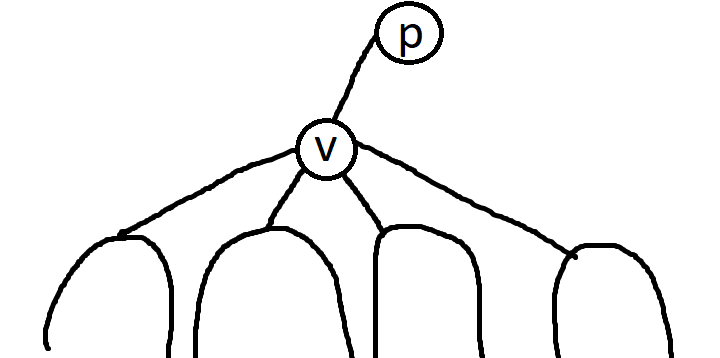
\includegraphics[width=5cm]{images/37_alg23.PNG}
\end{center}$\blacksquare \ $ \\
Теперь пусть v - вершина графа, \textbf{являющаяся корнем}. 
\\
\\
Тогда v - точка сочленения $\Longleftrightarrow$ из v выходит хотябы два древесных ребра\\
$\blacktriangle \ \leftarrow$ Между различными поддеревьями нет ребер, так как если бы ребро было, то эти два поддерева склеились бы в одно. Значит, после удаления v поддеревья станут независимыми компонентами связности графа, а значит, v - точка сочленения. \\ $\rightarrow$ Пусть это не так, и у вершины всего один сын.  
\begin{center}
    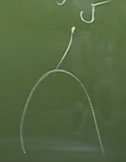
\includegraphics[width=3cm]{images/37_alg24.PNG}
\end{center}
Значит, удаление вершины v оставляет поддерево связной компонентой. (dfs запустился, как-то походил-походил и обошел все дерево, задействуя только одно ребро из v). Тогда v - не точка сочленения. Противоречие $\ \blacksquare$
\\
\\
\\
\\
\\
\begin{verbatim}
void dfs(int v, int p=-1){
    tin[v] = timer++;
    ret[v] = tin[v];
    used[v] = true;
    int cld = 0;
    
    for(int to:g[v]){
        if(to == p) continue;
        
        if(used[to]){
            ret[v] = min(ret[v], tin[to]);
        }else{
            cld++;
            dfs(to,v);
            ret[v] = min(ret[v], ret[to]);
            if(p != -1){
                if(ret[to] >= tin[v]) v - точка сочленения
            }else{
                if(cld >=2) v - точка сочленения
            }
        }
    }
}
\end{verbatim}